\documentclass{beamer}
\usepackage[utf8]{inputenc}
\usepackage{lmodern}
\usepackage[ngerman]{babel}
\usepackage{graphicx}
\usepackage{multicol}
\usepackage{listings}
%\usepackage{multimedia}
\usepackage{movie15}
\usepackage{hyperref}

\usetheme{Warsaw}
\usecolortheme{orchid} %ich weiß nicht mehr, ob warsaw standart orchid ist
\setbeamercovered{invisible}
\beamertemplatenavigationsymbolsempty %drecks command, macht die Navigationsleiste weg

\title{Simulation Ideen-Verbreitung}
\subtitle{Projektvorstellung}
\author{Arne Struck, Jonathan Werner, Manuel Börries}
\institute{Universität Hamburg, Fachschaft Informatik, Praktikum paralleles Programmieren}
\date{24. September 2014}


\begin{document}
\begin{frame}[plain]
	\titlepage
\end{frame}
	
%\begin{frame} {Gliederung}
%	\tableofcontents
%\end{frame}

\section{Projekt-Idee}
\begin{frame} {}
	(Grobe) Simulation von Entwicklung konkurrierender Ideen in einer begrenzten Welt.
\end{frame}

\section{Modellierung}


\begin{frame}
	\begin{columns}[T] % align columns
		\begin{column}{.73\textwidth}
			\begin{block} {Idee}
				\begin{itemize}
					\item Qualität
					\item Komplexität
					\item Weltanschauung
				\end{itemize}
			\end{block}
			\begin{block} {Mensch}
				\begin{itemize}
					\item Idee
					\item Weltanschauung
				\end{itemize}
			\end{block}
		\end{column}%
		\begin{column}{.18\textwidth}
		\begin{picture}(0,0)
			\put(-20,-130){
\includegraphics[scale=0.3]{finalPresentation/pics/Idee.png}}
		\end{picture}
		\end{column}%
	\end{columns}
\end{frame}

\begin{frame} {Welt \& Bewegung}

\end{frame}

\begin{frame} {Veränderung}
	
\end{frame}

\begin{frame} {Ablauf}
	\begin{itemize}
		\item Initialisierung des Feldes
		\item Zufälliger Spawn der Menschen mit mehrheitlich geringen Qualitätswerten
		\item Beginn der Simulationsschleife für \(n\) Schritte
		\begin{itemize}
			\item Mutationsevaluation
			\item Kommunikationsversuch
			\item Bewegung
		\end{itemize}
		\item Ende der Schleife
	\end{itemize}
\end{frame}

\section{Implementation}
\begin{frame}{Ideen}
placeholder
\end{frame}

\begin{frame} {Kommunikation \& Gewinner Berechnung}

\end{frame}

\begin{frame}{Parallelisierungsschema}
	\begin{picture}(0,230)
		\put(-120,0){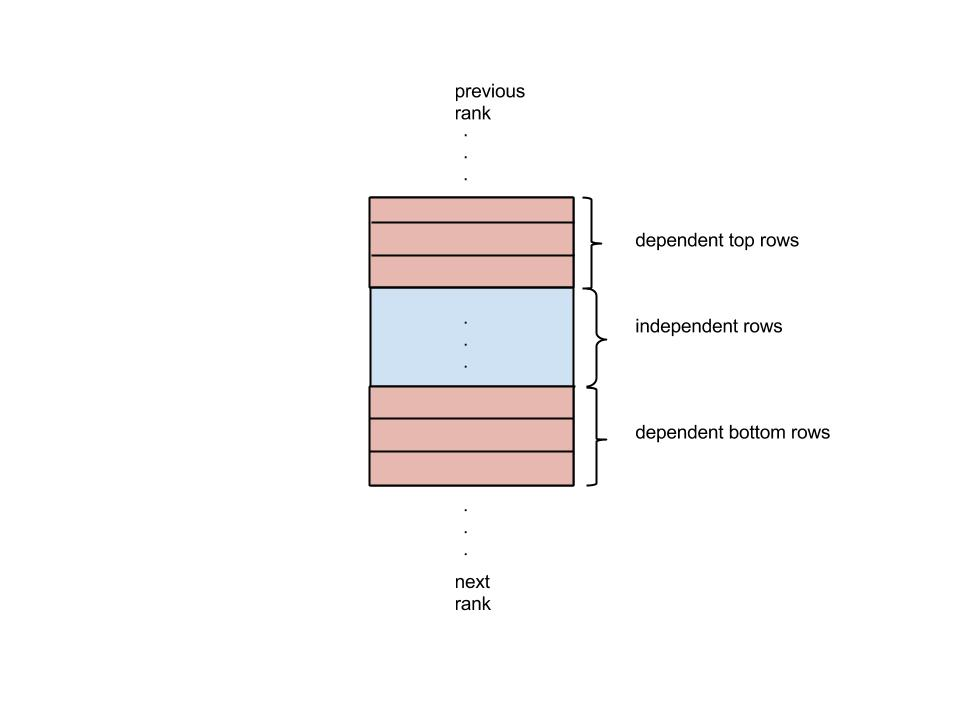
\includegraphics[height=8cm]{finalPresentation/pics/dependent-rows.jpg}}
		\put(170,180){\begin{minipage}[t]{0.4\linewidth}{
			\begin{itemize}
				\item for additional text	
			\end{itemize}
			}
		\end{minipage}}
	\end{picture}
\end{frame}

\begin{frame} {}
placeholder
\end{frame}
\section{Resultate und Messungen}
\begin{frame} {Profiling}
	HIER EIN BILD VON MESSUNGEN
\end{frame}

\begin{frame} {Tracing}
	idk, ob wir das machen wollen
\end{frame}

\begin{frame} {Ablauf}
	HIER BITTE EIN GUTES ABLAUF-GIF PLS
\end{frame}

\begin{frame} {Ergebnisse}
	\begin{itemize}
		\item Qualität nimmt über die Zeit zu
		\item Obwohl andere selten vollständig entfernt bilden 2-3 Ideen eine Majorität aus
		\item Qualität/Elaboriertheit nimmt über die Zeit zu
		\item Es bleiben einige Menschen mit Ideen niedriger Qualität
		\item Selten: Durch Mutation entwickelt sich eine verdrängte Idee zur dominanten
	\end{itemize}
\end{frame}
\section{Probleme und Lösungen}

\begin{frame}{Probleme}
	\begin{block}{Probleme beim Debuggen}
		\begin{itemize}
			\item Logik und Bewegung größtenteils unter Beteiligung von Zufallselementen
			\item oft nicht reproduzierbare Bugs 
		\end{itemize}
	\end{block}
	
	\begin{block} {Real-Time Visualisierung}
		\begin{itemize}
			\item große Datenmenge
			\item Uns war nicht klar wie/ob X-Forwarding mit dem Cluster funktioniert wird
		\end{itemize}
	\end{block}
\end{frame}


	

\end{document}
